\documentclass[11pt]{article}
\usepackage[margin=1in]{geometry}
\usepackage{amsmath,amssymb,graphicx,microtype,booktabs}
\usepackage[font=small,skip=3pt]{caption}
\usepackage[hidelinks]{hyperref}
\usepackage{enumitem}
\usepackage{tcolorbox}
\setlist{nosep,leftmargin=1.2em}
\newtcolorbox{intuitionbox}{
  colback=black!4,
  colframe=black!18,
  coltext=black!78,
  boxrule=0.45pt,
  arc=2pt,
  left=7pt,right=7pt,top=5pt,bottom=5pt,
  before skip=5pt,after skip=5pt,
  fonttitle=\small\sffamily\bfseries,
  fontupper=\small,
  coltitle=black!68,
  title={Intuitive interpretation}
}
\setlength{\parindent}{0pt}
\setlength{\parskip}{2.5pt plus 1pt minus 1pt}
\setlength{\textfloatsep}{5pt plus 2pt minus 2pt}
\setlength{\intextsep}{7pt plus 2pt minus 2pt}
\title{\vspace{-1.6em}\textbf{The Infrastructure--Isolation Principle}\vspace{-0.5em}}
\author{J. R. Landers\\[-1pt]\small Reliance, semantic neighborhoods, and proof complexity in Mathlib}
\date{\vspace{-1.2em}}

\begin{document}
\maketitle
\vspace{-1.6em}

A formal library grows by reuse.  Definitions support lemmas, lemmas support later theorems, and
automation hides long chains of accumulated infrastructure behind short tactic scripts.  This
suggests two competing pictures of maturity.  Reuse could make deep results resemble one another:
shared machinery might concentrate the library into dense families.  Or reuse could enable
specialization: common infrastructure might support increasingly particular endpoints whose proofs
have few close analogues.

Measurements on 10,000 theorem--proof pairs from LeanDojo Benchmark 4 support the second picture
\cite{leandojo}.  Theorems resting on more kernel-visible infrastructure have more involved recorded
proofs, but smaller semantic neighborhoods.  The contraction is stronger for proofs than for
statements.  We call this joint pattern the \emph{Infrastructure--Isolation Principle}:

\begin{quote}
\emph{In a mature formal library, declarations that depend on more mathematical infrastructure
tend to have more involved proofs but fewer close semantic peers; procedural specialization
outpaces semantic specialization.}
\end{quote}

\begin{intuitionbox}
The dependency graph measures how much mathematical scaffolding a theorem stands on.  The
embeddings measure how many close companions it has, and the complexity score measures how
involved its recorded construction is.  The surprise is that more scaffolding accompanies fewer
companions---especially for proofs.  This is an empirical pattern, not a theorem of Lean.
\end{intuitionbox}

\paragraph{Reliance in the kernel graph.}
Let $G=(V,E)$ be the directed graph of declarations in the pinned Mathlib environment.  An edge
$u\to v$ means that declaration $v$ uses constant $u$ in its kernel-checked type or value, including
the elaborated proof term.  The export contains 888,992 declarations and 13,264,773 direct edges.
Unlike identifiers written visibly in tactic syntax, these edges include constants introduced by
automation such as \texttt{simp}.

This graph-first view is also entering learned proving.  Graph2Tac builds hierarchical
representations of new formal concepts from the dependency structure of a Coq development and
updates them online as the library grows \cite{graph2tac}.  Here the graph becomes an object of
measurement in its own right: not only a route to the next tactic, but a record of how accumulated
infrastructure positions a theorem.

For target declaration $i$, let $A(i)$ contain every upstream declaration that can reach $i$, and
let $d(u,i)$ be the length of the shortest directed path from $u$ to $i$.  With discount
$0<\alpha\leq1$, define dependency mass and its reported reliance score by
\[
 D_\alpha(i)=\sum_{u\in A(i)}\alpha^{d(u,i)},
 \qquad R_i=\log\!\left(1+D_{0.5}(i)\right).
\]
Here $\log$ is the natural logarithm.  At $\alpha=1$, dependency mass counts distinct ancestors;
$\alpha=0.5$ emphasizes nearby infrastructure without discarding the transitive closure.  All
10,000 searches terminate within 52 levels.  The median target has 39 direct dependencies,
shortest-path depth 18, and $R_i=4.668$.

\paragraph{Connectedness in two semantic spaces.}
The same Cohere Embed v4 map used in the earlier semantic study sends statement text and proof text
separately to vectors $e_i^{(S)},e_i^{(P)}\in\mathbb{R}^{1024}$ \cite{statements}.  For view
$v\in\{S,P\}$, normalize
\[
 x_i^{(v)}=\frac{e_i^{(v)}}{\lVert e_i^{(v)}\rVert_2},
 \qquad \lVert e\rVert_2=\left(\sum_k e_k^2\right)^{1/2}.
\]
The dot product $x_i^{(v)}\mathbin{\cdot}x_j^{(v)}$ is then cosine similarity.  Let
$\mathcal N_{100}^{(v)}(i)$ be the exact top-100 neighbors of $i$ in view $v$.  A view-specific
threshold $\tau_v$ is the 99th percentile of 500,000 fixed random-pair cosines: $\tau_S=0.690$
and $\tau_P=0.755$.  For $j\in\mathcal N_{100}^{(v)}(i)$, set
\[
 w_{ij}^{(v)}=\max\!\left\{0,
 x_i^{(v)}\mathbin{\cdot}x_j^{(v)}-\tau_v\right\},\qquad
 p_{ij}^{(v)}=\frac{w_{ij}^{(v)}}{\sum_{\ell\in\mathcal N_{100}^{(v)}(i)}w_{i\ell}^{(v)}}.
\]
The effective semantic neighborhood is
\[
 S_i^{(v)}=\exp\!\left(-\sum_{j\in\mathcal N_{100}^{(v)}(i)}
 p_{ij}^{(v)}\log p_{ij}^{(v)}\right),
\]
with $S_i^{(v)}=0$ if every weight is zero.  This is the entropy-equivalent number of neighbors
sharing the retained similarity weight: one dominant neighbor gives a value near one, and many
balanced neighbors give a larger value, capped here at 100.  Median connectedness is 31.3 in
statement space but only 8.6 in proof space.

\paragraph{Complexity of the recorded proof.}
Let $s_i$ be tactic-step count, $r_i$ direct kernel-reference count, $h_i$ maximum dependency
depth, and $q_{it}$ the fraction of proof steps whose tactic head is $t$.  Tactic-head entropy is
$H_i=-\sum_tq_{it}\log q_{it}$.  If
$z(y)=(y-\bar y)/\operatorname{sd}(y)$ standardizes a component over the 10,000 targets, define
\[
 C_i=\frac14\left[
 z\!\left(\log(1+s_i)\right)+z\!\left(\log(1+r_i)\right)+z(h_i)+z(H_i)
 \right].
\]
Thus $C_i$ is an equal-weight index of observed structural involvement.  It is not proof length
alone, and it is not a claim about intrinsic mathematical difficulty.

\begin{figure}[t]
  \centering
  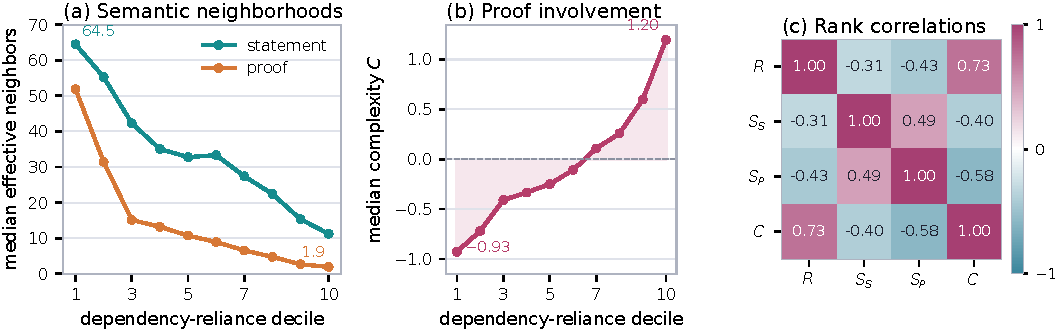
\includegraphics[width=\textwidth]{infrastructure_isolation.pdf}
  \caption{The Infrastructure--Isolation Principle in the frozen 10,000-target sample.
  Equal-count reliance deciles show (a) shrinking statement and proof neighborhoods and
  (b) increasing proof complexity.  Panel (c) gives Spearman rank correlations among reliance
  $R$, statement connectedness $S_S$, proof connectedness $S_P$, and complexity $C$.
  Effective neighborhood medians, rather than embedding projections, are shown.}
  \label{fig:principle}
\end{figure}

\paragraph{The empirical sign pattern.}
Write $\rho(X,Y)$ for Spearman rank correlation, the ordinary Pearson correlation of the ranks of
$X$ and $Y$.  The central observation is
\[
 \rho(R,C)=0.734>0,
 \qquad
 \rho(R,S_P)<\rho(R,S_S)<0,
 \qquad
 \rho(C,S_P)<\rho(C,S_S)<0,
\]
with measured values
\[
 \rho(R,S_S)=-0.314,\quad \rho(R,S_P)=-0.431,
 \qquad
 \rho(C,S_S)=-0.398,\quad \rho(C,S_P)=-0.584.
\]
Statement and proof connectedness remain positively but incompletely aligned:
$\rho(S_S,S_P)=0.490$.  The pattern is therefore not ``everything difficult is far from
everything else.''  It says that structural accumulation and semantic density point in opposing
directions, while statement and proof geometries preserve a partial bridge.

The positive $R$--$C$ association is partly built into the definitions: $C$ contains direct
reference count and dependency depth.  The negative connectedness associations are not.  Neither
$S_S$ nor $S_P$ uses the dependency graph or tactic counts.  They supply the nontrivial half of the
principle.

\paragraph{Proposition (the infrastructure rank-sign law).}
Let $U_X=\Pr(X'<X)+\tfrac12\Pr(X'=X)$ be the population midrank of
$X\in\{R,C,S_S,S_P\}$.  Suppose a latent infrastructure coordinate $Z$ makes
$m_X(z)=\mathbb E[U_X\mid Z=z]$ nondecreasing for $X=R,C$ and nonincreasing for
$X=S_S,S_P$.  If the rank residuals are pairwise conditionally uncorrelated given $Z$, then
\[
 \rho(R,C),\ \rho(S_S,S_P)\geq0,
 \qquad \rho(A,B)\leq0
 \quad\text{for }A\in\{R,C\},\ B\in\{S_S,S_P\}.
\]
\emph{Proof.}
Total covariance reduces the left side below to the right; for an independent $Z'$,
\[
 2\operatorname{Cov}(U_X,U_Y)
 =\mathbb E[(f(Z)-f(Z'))(g(Z)-g(Z'))].
\]
Here $f=m_X$ and $g=m_Y$.  The product has the sign claimed when the functions move in the same
or opposite directions; rank standardization preserves it.  Strict sign on a positive-probability
set gives strict inequality. $\square$

\begin{intuitionbox}
Imagine moving along one hidden ``infrastructure'' dial.  Reliance and complexity rise as the dial
turns, while both kinds of neighborhood shrink.  That alone forces the observed correlation
directions.  It does not determine how strong the correlations should be, and the faster isolation
of proofs remains empirical.
\end{intuitionbox}

\paragraph{Corollary (the one-factor tetrad test).}
Specialize further to standardized rank variables
\[
 \widetilde U_R=a_RZ+\varepsilon_R,\quad
 \widetilde U_C=a_CZ+\varepsilon_C,\quad
 \widetilde U_{S_S}=-a_SZ+\varepsilon_S,\quad
 \widetilde U_{S_P}=-a_PZ+\varepsilon_P,
\]
where $a_R,a_C,a_S,a_P>0$, $\operatorname{Var}(Z)=1$, and the residuals are mutually uncorrelated
and uncorrelated with $Z$.  Pairwise correlations are then signed products of loadings, so
\[
 \rho(R,C)\rho(S_S,S_P)
 =\rho(R,S_S)\rho(C,S_P)
 =\rho(R,S_P)\rho(C,S_S).
\]
\begin{intuitionbox}
If one linear hidden dial controlled everything, the three correlation products would agree.  They
do not: the measured values are $0.360$, $0.183$, and $0.172$.  One dial therefore explains the
directions but not their strengths.  Nonlinearity, correlated residual structure, or an additional
procedural axis is needed to explain the remaining geometry.
\end{intuitionbox}

\paragraph{A gradient, not only a correlation.}
Figure~\ref{fig:principle} orders targets by $R_i$ and divides them into ten equal-count groups.
From lowest to highest decile, median statement neighborhood falls from 64.5 to 11.2, proof
neighborhood from 51.9 to 1.9, and complexity rises from $-0.93$ to $1.20$.  Proof connectedness
decreases at every step; statement connectedness has one small reversal.  Rankings remain stable:
tested dependency discounts correlate at least $0.904$, semantic thresholds at least $0.926$, and
leave-one-component-out complexity scores at least $0.941$ with the primary rankings.

\paragraph{Why proofs isolate faster than statements.}
Statements belong to recurring mathematical families; recorded tactic proofs are implementations
shaped by available lemmas, automation, notation, and intermediate goals.  Common infrastructure
can support similar claims without enforcing similar proof artifacts.  Earlier feature topics and
embeddings separated content from procedure while retaining a local bridge \cite{textures,statements}.
The present result adds direction from the kernel graph: increasing dependency depth weakens both
neighborhoods, but weakens the procedural one more.  Lean Copilot already places tactic suggestion,
proof search, and premise selection behind one Lean-native learned interface \cite{leancopilot}; our
measurements suggest that such systems may benefit from treating semantic family and procedural
precedent as related but distinct retrieval signals.

\paragraph{A two-axis map.}
Reliance and connectedness distinguish reusable basics, unusual elementary results, mature
specialized families, and bespoke endpoints atop deep infrastructure.  The last is a retrieval
frontier: semantic examples can help generation \cite{nearby}, but a high-reliance, low-connectedness
theorem needs broad library concepts while offering few procedural precedents.  Retrieval for this
tail should combine semantic proximity with dependency coverage.  LeanSearch v2 sharpens the same
frontier as \emph{global premise retrieval}: recovering a scattered supporting set rather than one
nearest declaration \cite{leansearchv2}.

\paragraph{Scope of the principle.}
These scores describe one snapshot, one recorded proof per theorem, and one encoder.  Dependency
mass includes formalization machinery; scripts are not canonical; neighborhoods are model-dependent;
and the analysis is observational.  Replication across snapshots, libraries, and multiple proofs
should test the principle.  Within those limits, the result joins structural and learned geometry:
common foundations support specialized conclusions whose proof artifacts become distinctive faster
than their statements do.  Accumulated infrastructure produces specialization, not homogenization.

\begin{thebibliography}{9}\scriptsize
\setlength{\itemsep}{0pt}
\bibitem{textures} J. R. Landers. ``Textures of Modern Formal Mathematics.'' 2026.
\bibitem{statements} J. R. Landers. ``What Statements Know, What Proofs Do.'' 2026.
\bibitem{nearby} J. R. Landers. ``Nearby Examples, New Proofs.'' 2026.
\bibitem{leandojo} K. Yang et al. ``LeanDojo: Theorem Proving with Retrieval-Augmented Language Models.'' NeurIPS, 2023.
\bibitem{graph2tac} L. Blaauwbroek et al. ``Graph2Tac: Online Representation Learning of Formal Math Concepts.'' 2024.
\bibitem{leancopilot} P. Song, K. Yang, and A. Anandkumar. ``Towards Large Language Models as Copilots for Theorem Proving in Lean.'' 2024.
\bibitem{leansearchv2} G. Gao et al. ``LeanSearch v2: Global Premise Retrieval for Lean 4 Theorem Proving.'' 2026.
\end{thebibliography}

\end{document}
